% Gráfico: Taxa de Destruição - Média de Nós Restantes
\begin{figure}[htbp]
\centering
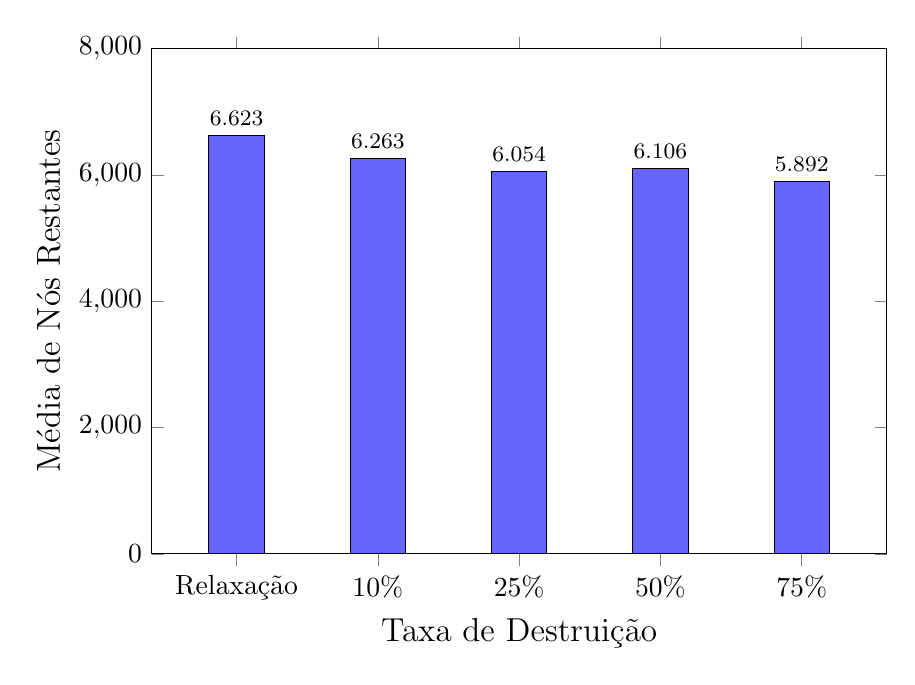
\begin{tikzpicture}
\begin{axis}[
    ybar,
    bar width=20pt,
    width=0.9\textwidth,
    height=8cm,
    ylabel={Média de Nós Restantes},
    xlabel={Taxa de Destruição},
    symbolic x coords={Relaxação, 10\%, 25\%, 50\%, 75\%},
    xtick=data,
    nodes near coords,
    nodes near coords align={vertical},
    nodes near coords style={font=\footnotesize},
    every node near coord/.append style={/pgf/number format/fixed,
        /pgf/number format/precision=0,
        /pgf/number format/use comma},
    ymin=0,
    ymax=8000,
    enlarge x limits=0.15,
    ylabel style={font=\large},
    xlabel style={font=\large},
    tick label style={font=\normalsize},
]
\addplot[fill=blue!60] coordinates {
    (Relaxação,6623)
    (10\%,6263)
    (25\%,6054)
    (50\%,6106)
    (75\%,5892)
};
\end{axis}
\end{tikzpicture}
\caption{Média de nós restantes na árvore de Branch-and-Bound para diferentes taxas de destruição do LNS. A configuração de 75\% apresentou a menor média, com 5.892 nós restantes por instância.}
\label{fig:avg_nodes_cand}
\end{figure}
